\documentclass{article}\usepackage{graphicx, color}
%% maxwidth is the original width if it is less than linewidth
%% otherwise use linewidth (to make sure the graphics do not exceed the margin)
\makeatletter
\def\maxwidth{ %
  \ifdim\Gin@nat@width>\linewidth
    \linewidth
  \else
    \Gin@nat@width
  \fi
}
\makeatother

\definecolor{fgcolor}{rgb}{0.2, 0.2, 0.2}
\newcommand{\hlnumber}[1]{\textcolor[rgb]{0,0,0}{#1}}%
\newcommand{\hlfunctioncall}[1]{\textcolor[rgb]{0.501960784313725,0,0.329411764705882}{\textbf{#1}}}%
\newcommand{\hlstring}[1]{\textcolor[rgb]{0.6,0.6,1}{#1}}%
\newcommand{\hlkeyword}[1]{\textcolor[rgb]{0,0,0}{\textbf{#1}}}%
\newcommand{\hlargument}[1]{\textcolor[rgb]{0.690196078431373,0.250980392156863,0.0196078431372549}{#1}}%
\newcommand{\hlcomment}[1]{\textcolor[rgb]{0.180392156862745,0.6,0.341176470588235}{#1}}%
\newcommand{\hlroxygencomment}[1]{\textcolor[rgb]{0.43921568627451,0.47843137254902,0.701960784313725}{#1}}%
\newcommand{\hlformalargs}[1]{\textcolor[rgb]{0.690196078431373,0.250980392156863,0.0196078431372549}{#1}}%
\newcommand{\hleqformalargs}[1]{\textcolor[rgb]{0.690196078431373,0.250980392156863,0.0196078431372549}{#1}}%
\newcommand{\hlassignement}[1]{\textcolor[rgb]{0,0,0}{\textbf{#1}}}%
\newcommand{\hlpackage}[1]{\textcolor[rgb]{0.588235294117647,0.709803921568627,0.145098039215686}{#1}}%
\newcommand{\hlslot}[1]{\textit{#1}}%
\newcommand{\hlsymbol}[1]{\textcolor[rgb]{0,0,0}{#1}}%
\newcommand{\hlprompt}[1]{\textcolor[rgb]{0.2,0.2,0.2}{#1}}%

\usepackage{framed}
\makeatletter
\newenvironment{kframe}{%
 \def\at@end@of@kframe{}%
 \ifinner\ifhmode%
  \def\at@end@of@kframe{\end{minipage}}%
  \begin{minipage}{\columnwidth}%
 \fi\fi%
 \def\FrameCommand##1{\hskip\@totalleftmargin \hskip-\fboxsep
 \colorbox{shadecolor}{##1}\hskip-\fboxsep
     % There is no \\@totalrightmargin, so:
     \hskip-\linewidth \hskip-\@totalleftmargin \hskip\columnwidth}%
 \MakeFramed {\advance\hsize-\width
   \@totalleftmargin\z@ \linewidth\hsize
   \@setminipage}}%
 {\par\unskip\endMakeFramed%
 \at@end@of@kframe}
\makeatother

\definecolor{shadecolor}{rgb}{.97, .97, .97}
\definecolor{messagecolor}{rgb}{0, 0, 0}
\definecolor{warningcolor}{rgb}{1, 0, 1}
\definecolor{errorcolor}{rgb}{1, 0, 0}
\newenvironment{knitrout}{}{} % an empty environment to be redefined in TeX

\usepackage{alltt}
\usepackage{mathtools}
\usepackage{amsfonts}
\usepackage{subfig}
\usepackage{float}
%\VignetteEngine{knitr}
%\VignetteIndexEntry{}
\IfFileExists{upquote.sty}{\usepackage{upquote}}{}

\begin{document}
\title{Random Portfolios}
\author{Mike Flynn, Angel Zhou, Dave Kane}
\maketitle

\section*{Introduction}




Imagine you have one thousand dollars that you want to invest in two stocks: General Electric (GE) and International Business Machines (IBM). You could invest 25 percent of your million dollars in GE and the remaining 75 percent in IBM, or, to present another scenario, you could halve your money and put five hundred thousand dollars into GE and five hundred thousand dollars into IBM. There is an endless amount of ways that you can invest one million dollars into the two stocks.

\begin{figure}[H]
\begin{knitrout}
\definecolor{shadecolor}{rgb}{0.969, 0.969, 0.969}\color{fgcolor}
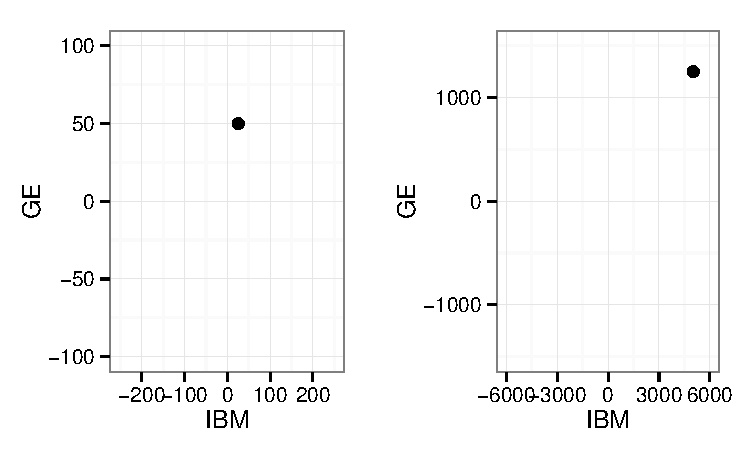
\includegraphics[width=\maxwidth]{figure/figure1} 

\end{knitrout}

\caption{Let's say your portfolio consists of 25 shares of IBM and 50 shares of GE. The plot on the left displays this coordinate in share space, meaning the x and y coordinates of the point represent the amount of shares invested in each stock. Alternatively, you can view the portfolio in dollar terms. This is done by multiplying the stock price by the number of shares, resulting in the total amount spent in each stock. The price of GE is currently at around 25 dollars apiece while the price of each IBM stock is approximately 200 dollars. Thus, 25 shares of IBM becomes 5,000 dollars and 50 shares of GE is valued at 1,250 dollars. The plot on the right displays the same portfolio as the one on the left, but plots the portfolio is in dollar space. This means that the x and y coordinates represent the total amount of money that you invested into each respective stock.}
\end{figure}

\begin{figure}[H]
\begin{knitrout}
\definecolor{shadecolor}{rgb}{0.969, 0.969, 0.969}\color{fgcolor}
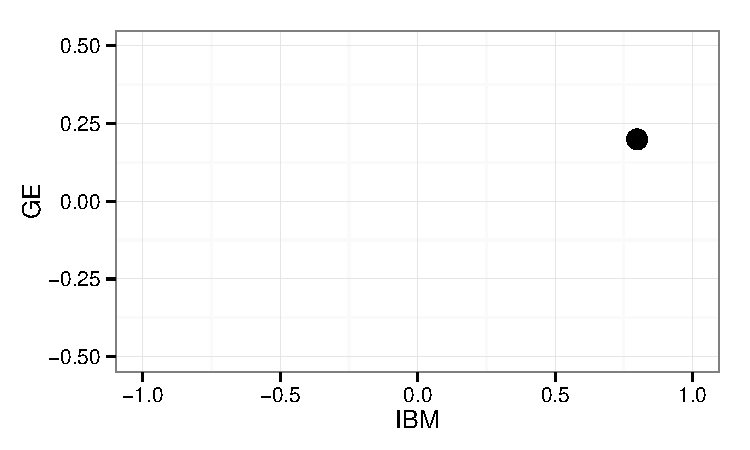
\includegraphics[width=\maxwidth]{figure/figure2} 

\end{knitrout}

\caption{The same portfolio as that in Figure 1 is replotted in portion space. In other words, this figure displays the portfolio where the x and y coordinates represent the percentage of the total amount of money that is invested into each respective stock. To use the same example as before, since you spent 5,000 dollars on IBM and 1,250 dollars on GE, you expended a total of 6,250 dollars. $1250/6250 = 0.2$, so 20 percent of your budget is spent in GE. Transitively, and 80 percent is spent on IBM. These percentages are plotted in decimal form in the figure. In this document, we will be referring to portfolios plotted in portion space.}
\end{figure}

As mentioned before, there are an infinite amount of ways to split the invested money. Earlier we thought about dividing the money in dollar terms. Now let's think about it in percentages in decimal form. No matter how you split the money, whether you put .5 in IBM and .5 in GE, or .2 in IBM and .8 in GE, the two values must sum to 1, or 100 percent. In other words, this portfolio is fully invested; no money is put aside for other uses.
In order to visualize how all the possible portfolios would appear in a 2-D space, you can generate random weights, creating a random way of splitting the money. When generating random weights, the sum of the variables $x + y = 1$ and ${x, y} > 0$.

\begin{figure}[H]
\begin{knitrout}
\definecolor{shadecolor}{rgb}{0.969, 0.969, 0.969}\color{fgcolor}
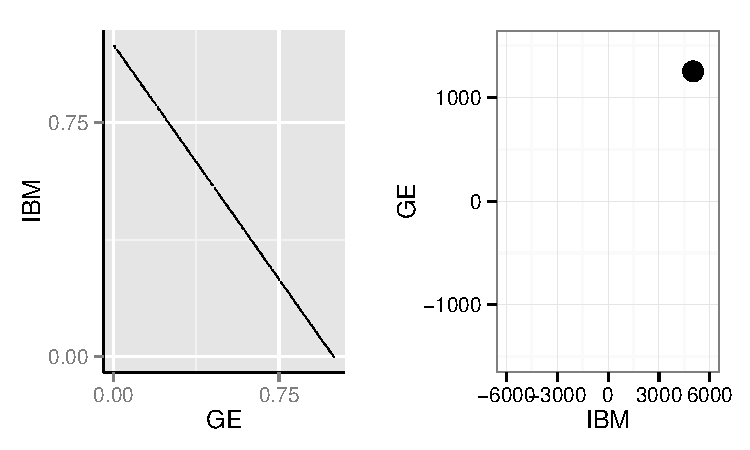
\includegraphics[width=\maxwidth]{figure/figure3} 

\end{knitrout}

\caption{1,000 random samples of two stocks were taken, where each stocks' value represents the percentage of the total money that is invested in each stock. The two percentages are represented in decimal form, thus summing to one. The result is a diagonal line from the points (0,1) to (1,0). Each point on this line represents a possible portfolio.}
\end{figure}

Now let's say that you want to add Coca-Cola (KO) to the stocks that you are investing in. Now that you have three stocks, you must generate three random weights that sum to 1. For example, you could invest .3, .3, and .4 of your total funding in KO, GE, and IBM respectively. 
  
\begin{figure}[H]
\begin{knitrout}
\definecolor{shadecolor}{rgb}{0.969, 0.969, 0.969}\color{fgcolor}
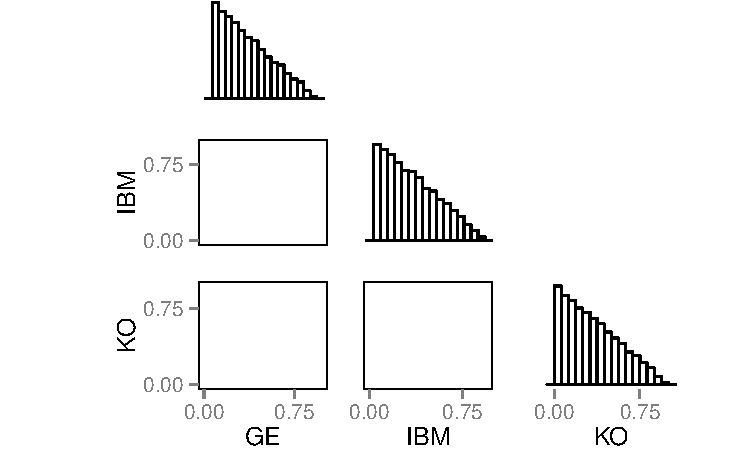
\includegraphics[width=\maxwidth]{figure/figChunk1} 

\end{knitrout}

\caption{Random weights were sampled for Google (GE), Coca-Cola (KO), and International Business Machines (IBM). Each set of randomly sampled weights for the three stocks all sum to 1. The pairwise scatterplots display the same distribution of 1000 random weights, and shows that they were of the same distribution. Additionally, the maximum sum for the weight distributions for any two variables is 1, and the minimum sum is 0. On the diagonal above the three scatterplots are three histograms. They represent density plots of 10,000 randomly sampled weights. The histograms display the distributions of the variables and indicate that the most likely value for any given variable is close to 0.}
\end{figure}

\begin{figure}[H]
\begin{knitrout}
\definecolor{shadecolor}{rgb}{0.969, 0.969, 0.969}\color{fgcolor}

\includegraphics[width=\maxwidth]{figure/fiveByFiveGrid} 

\end{knitrout}

\caption{1000 random samples.}
\end{figure}

\section*{hitandrun()}

Random points were generated in order to create the data for the previous two figures. The function used to create the random weights is called "hitandrun".

\begin{figure}[H]
\begin{knitrout}
\definecolor{shadecolor}{rgb}{0.969, 0.969, 0.969}\color{fgcolor}
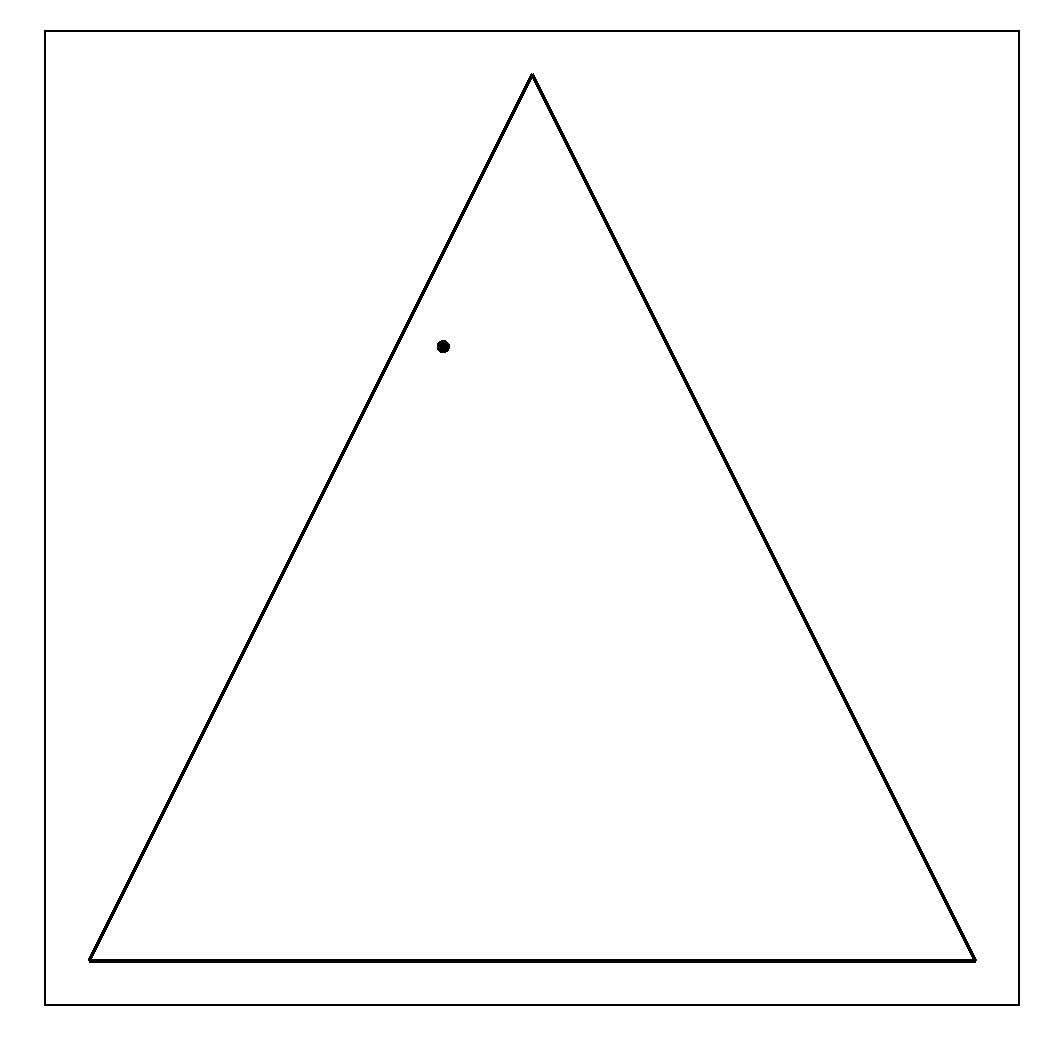
\includegraphics[width=\maxwidth]{figure/hitandrun_walkthrough1} 

\end{knitrout}

\caption{There are a number of steps within the function, the first of which is that it picks a random point within a simplex.}
\end{figure}

\begin{figure}[H]
\begin{knitrout}
\definecolor{shadecolor}{rgb}{0.969, 0.969, 0.969}\color{fgcolor}
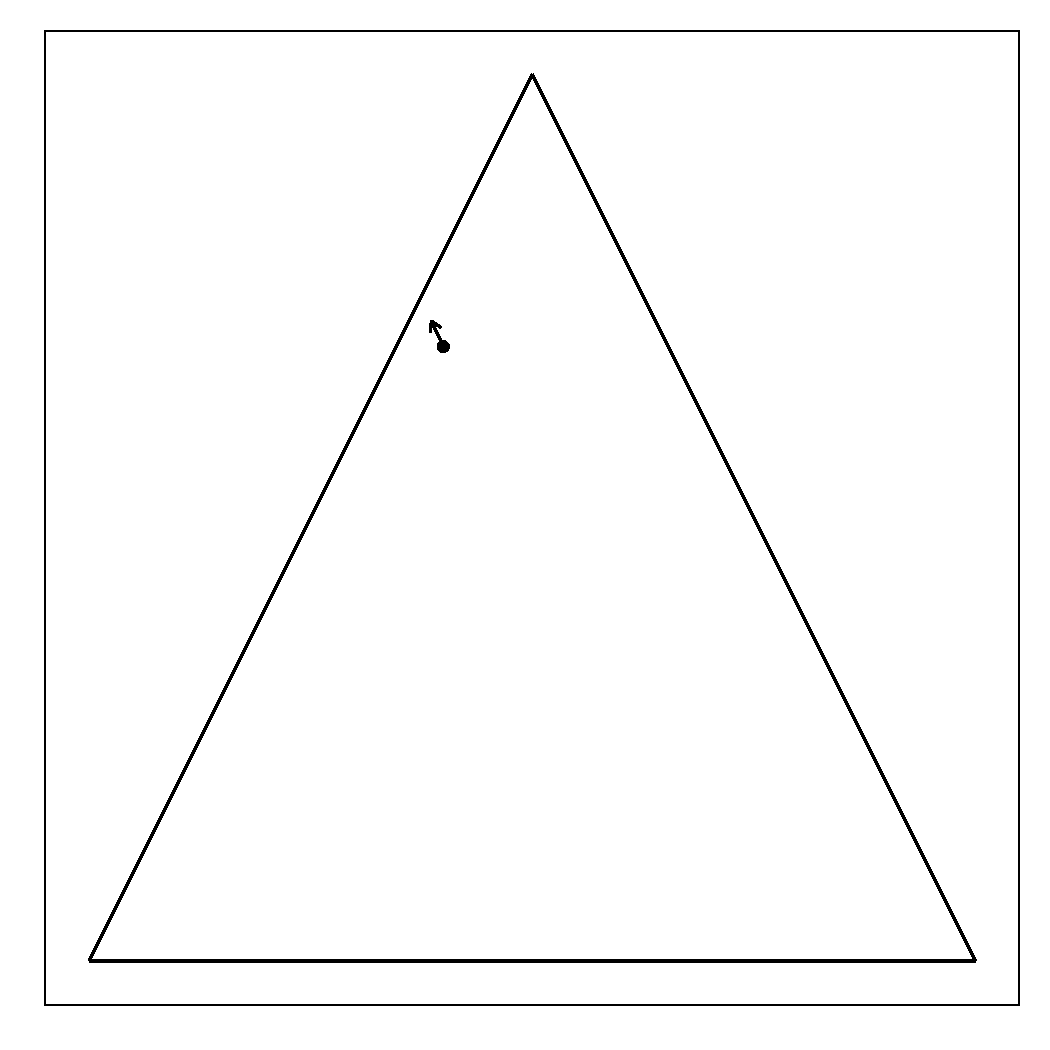
\includegraphics[width=\maxwidth]{figure/hitandrun_walkthrough2} 

\end{knitrout}

\caption{Next, hitandrun() picks a random direction, as shown by the arrow.}
\end{figure}

\begin{figure}[H]
\begin{knitrout}
\definecolor{shadecolor}{rgb}{0.969, 0.969, 0.969}\color{fgcolor}
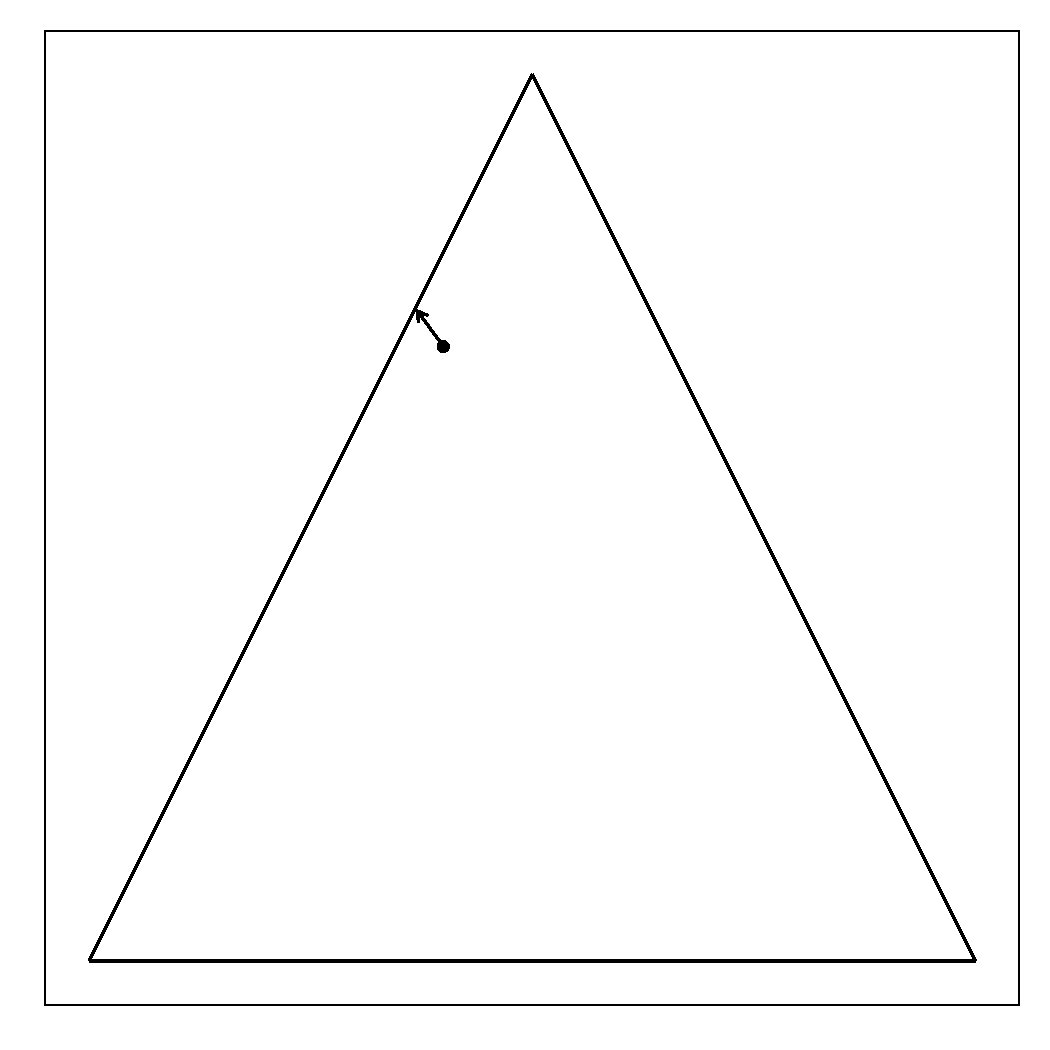
\includegraphics[width=\maxwidth]{figure/hitandrun_walkthrough3} 

\end{knitrout}

\caption{The function then extends that arrow until it hits an edge of the simplex.}
\end{figure}

\begin{figure}[H]
\begin{knitrout}
\definecolor{shadecolor}{rgb}{0.969, 0.969, 0.969}\color{fgcolor}
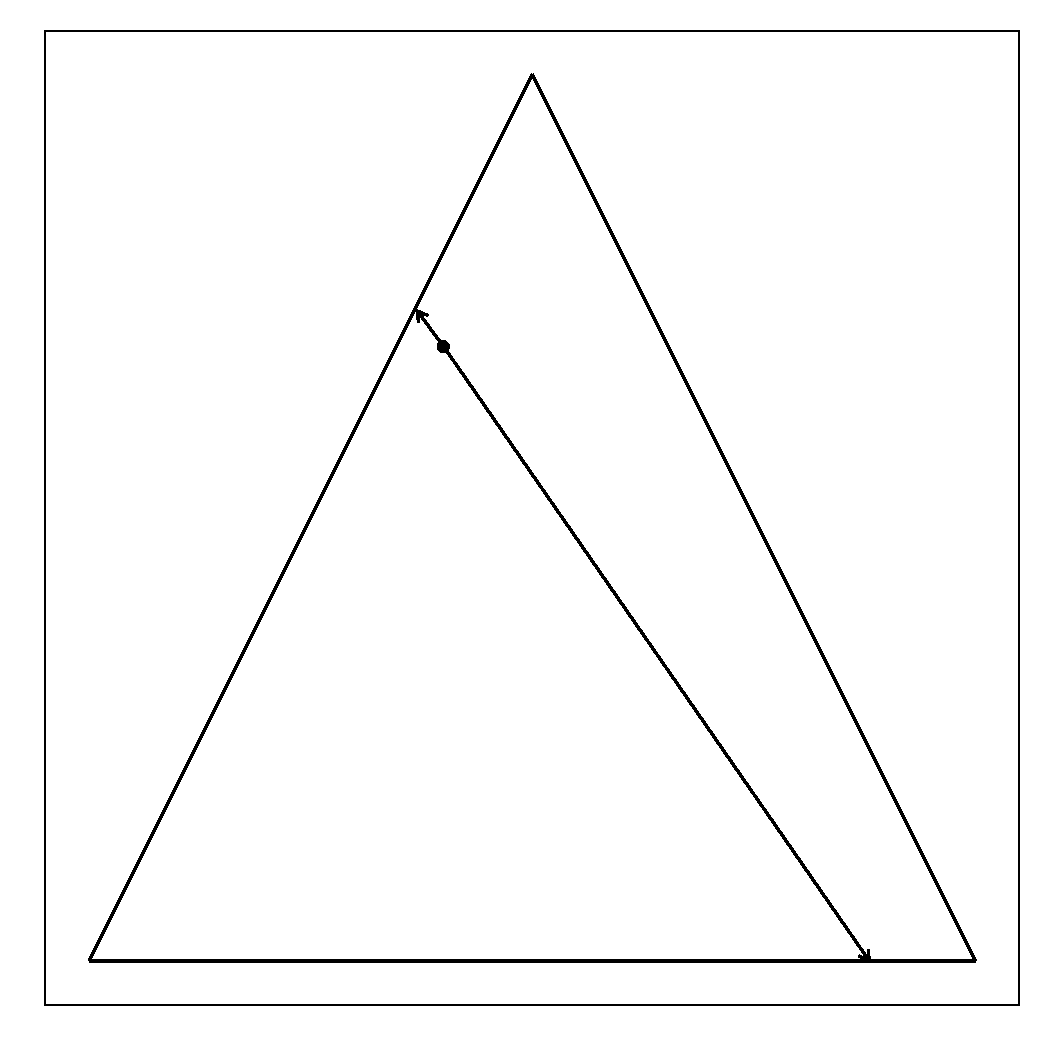
\includegraphics[width=\maxwidth]{figure/hitandrun_walkthrough4} 

\end{knitrout}

\caption{Next, hitandrun() extends the arrow in the other direction until it hits another point on the edge of the simplex.}
\end{figure}

\begin{figure}[H]
\begin{knitrout}
\definecolor{shadecolor}{rgb}{0.969, 0.969, 0.969}\color{fgcolor}
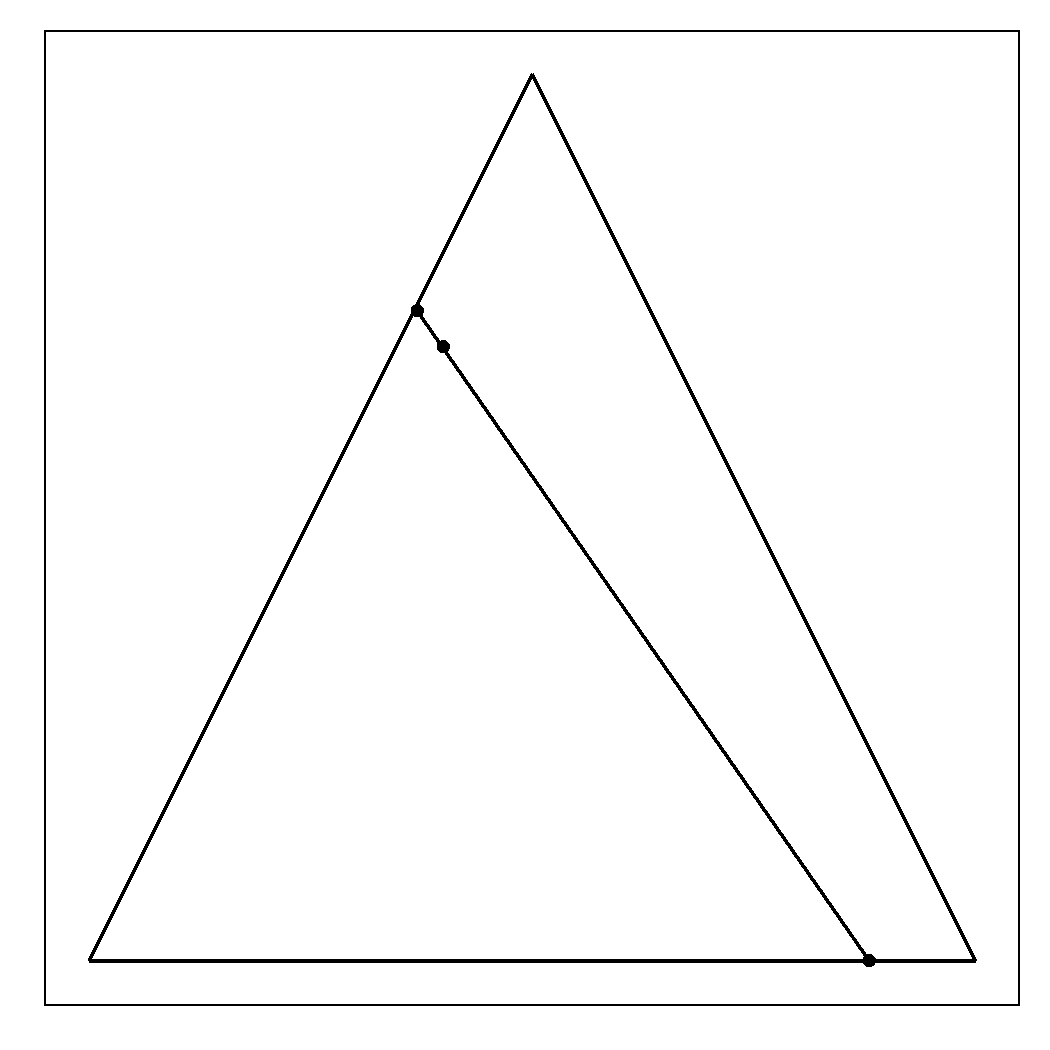
\includegraphics[width=\maxwidth]{figure/hitandrun_walkthrough5} 

\end{knitrout}

\caption{A line segment is formed. It passes through the initial point and connects the two points where the directional arrows intersected the simplex.}
\end{figure}

\begin{figure}[H]
\begin{knitrout}
\definecolor{shadecolor}{rgb}{0.969, 0.969, 0.969}\color{fgcolor}
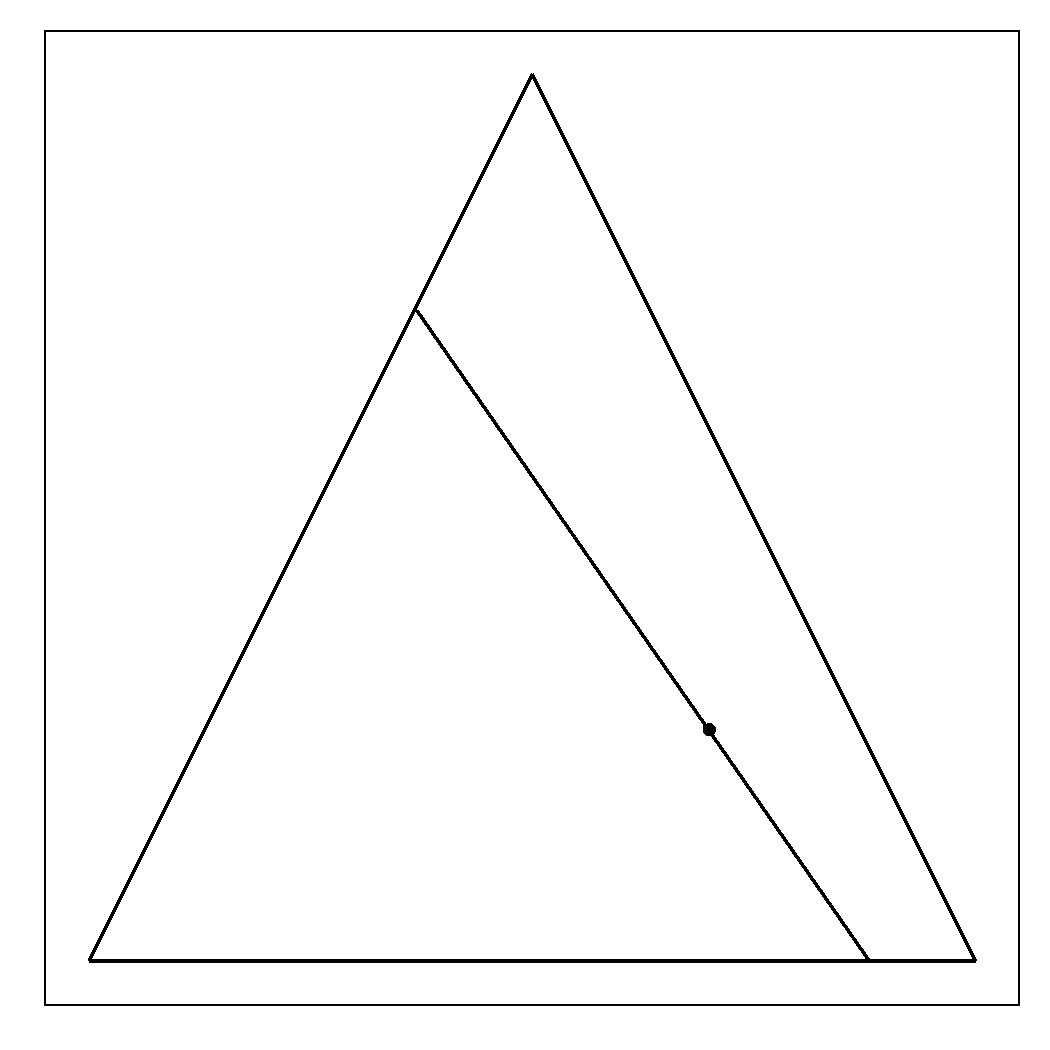
\includegraphics[width=\maxwidth]{figure/hitandrun_walkthrough6} 

\end{knitrout}

\caption{Finally, a random point is picked on the line segment shown in figure 10.}
\end{figure}

\begin{figure}[H]
\begin{knitrout}
\definecolor{shadecolor}{rgb}{0.969, 0.969, 0.969}\color{fgcolor}
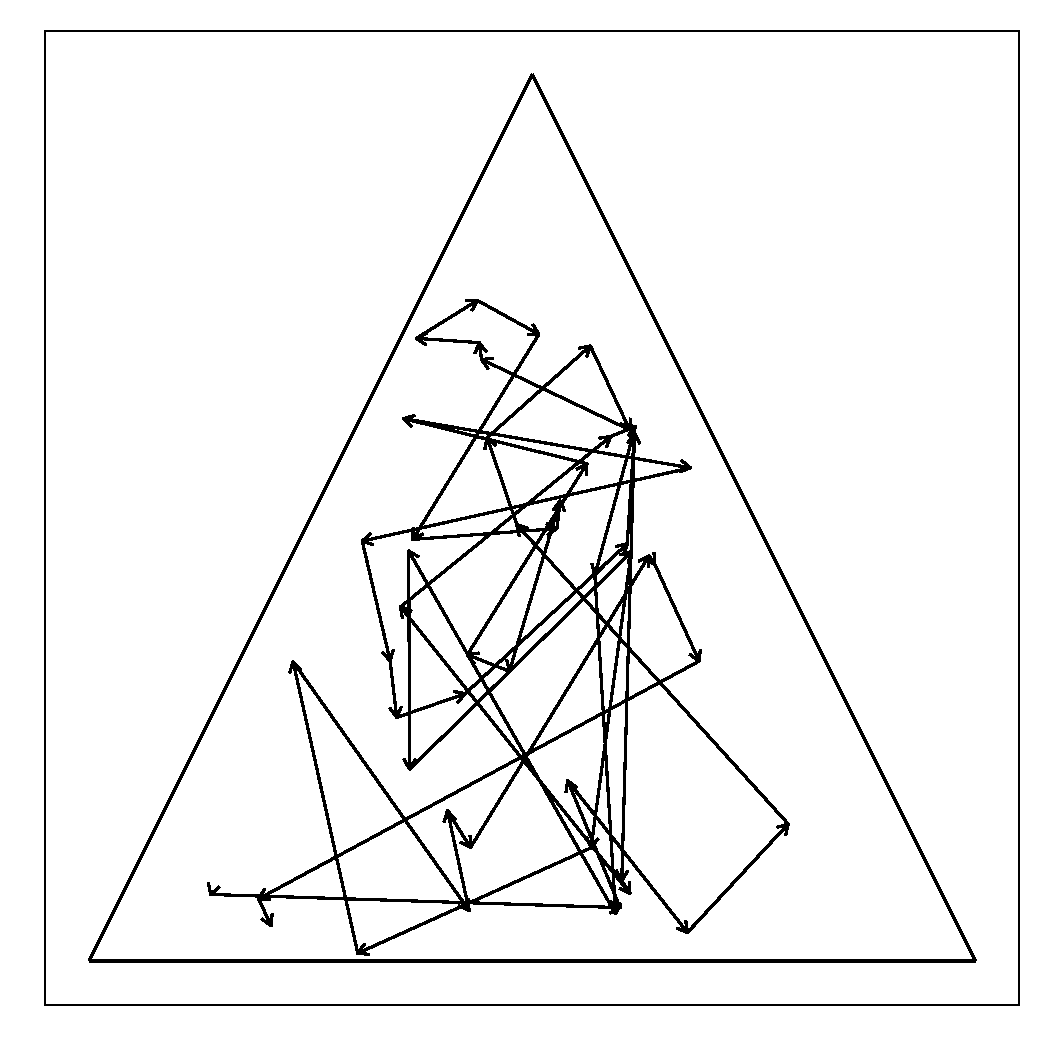
\includegraphics[width=\maxwidth]{figure/hitandrun_walkthrough7} 

\end{knitrout}

\caption{hitandrun() then repeats the previous steps, resulting in the creation of many points. This figure displays the outcome of 50 repetitions of the hitandrun algorithm that was just explained.}
\end{figure}

\section*{mirror()}

mirror() is another function used in the process of creating random portfolios.This function also consists of points jumping from one place to another.

\begin{figure}[H]
\begin{knitrout}
\definecolor{shadecolor}{rgb}{0.969, 0.969, 0.969}\color{fgcolor}
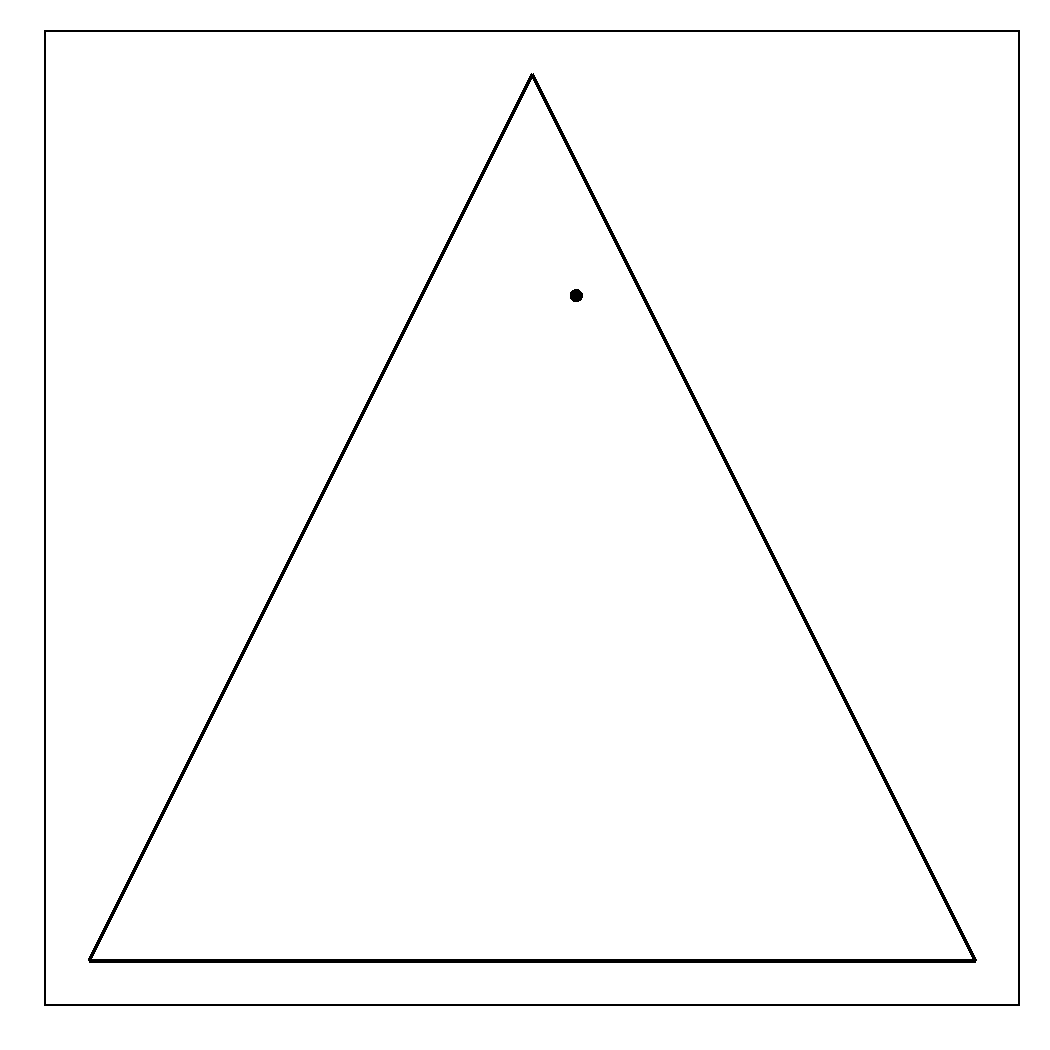
\includegraphics[width=\maxwidth]{figure/mirror_walkthrough1} 

\end{knitrout}

\caption{Similar to hitandrun(), mirror() begins by selecting a random point.}
\end{figure}

\begin{figure}[H]
\begin{knitrout}
\definecolor{shadecolor}{rgb}{0.969, 0.969, 0.969}\color{fgcolor}
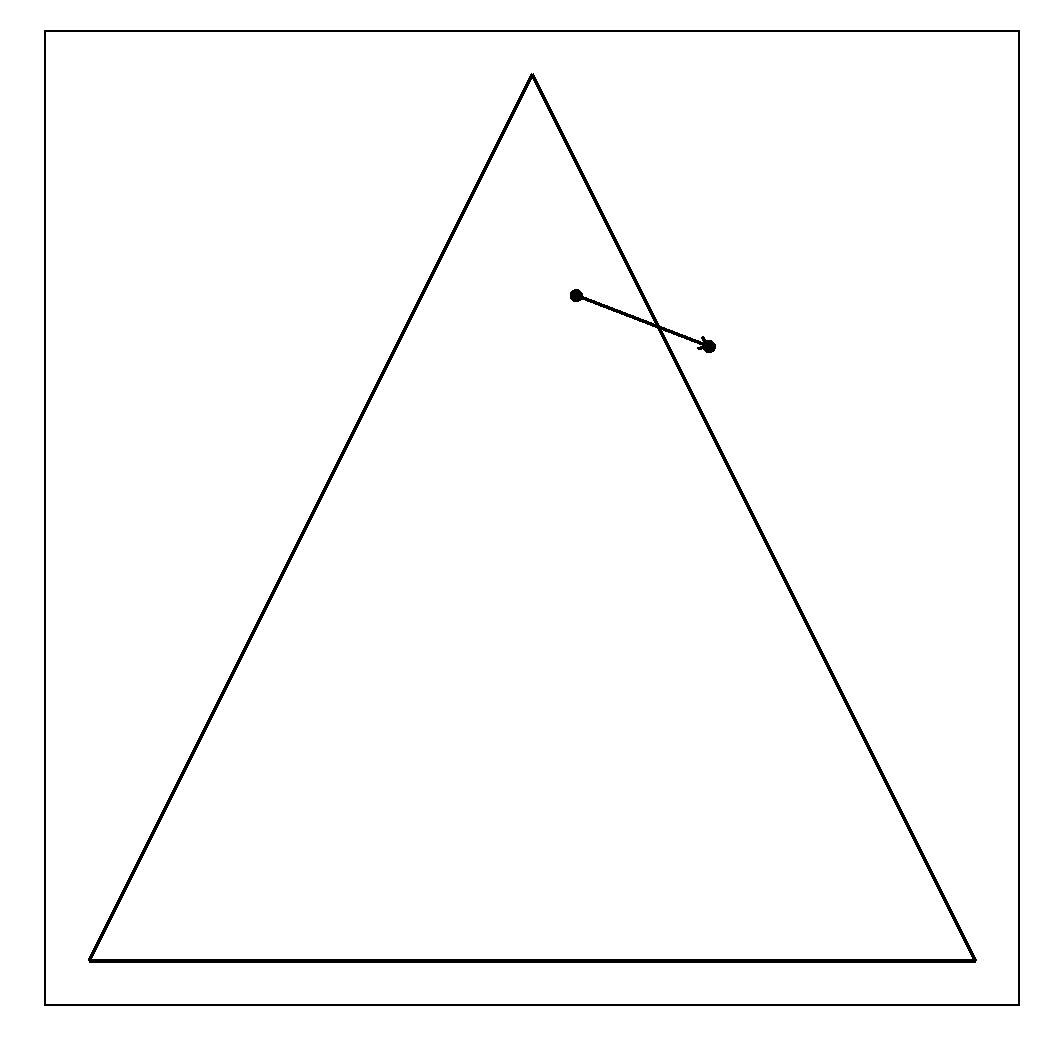
\includegraphics[width=\maxwidth]{figure/mirror_walkthrough2} 

\end{knitrout}

\caption{The point then jumps to a random place in space.}
\end{figure}

\begin{figure}[H]
\begin{knitrout}
\definecolor{shadecolor}{rgb}{0.969, 0.969, 0.969}\color{fgcolor}
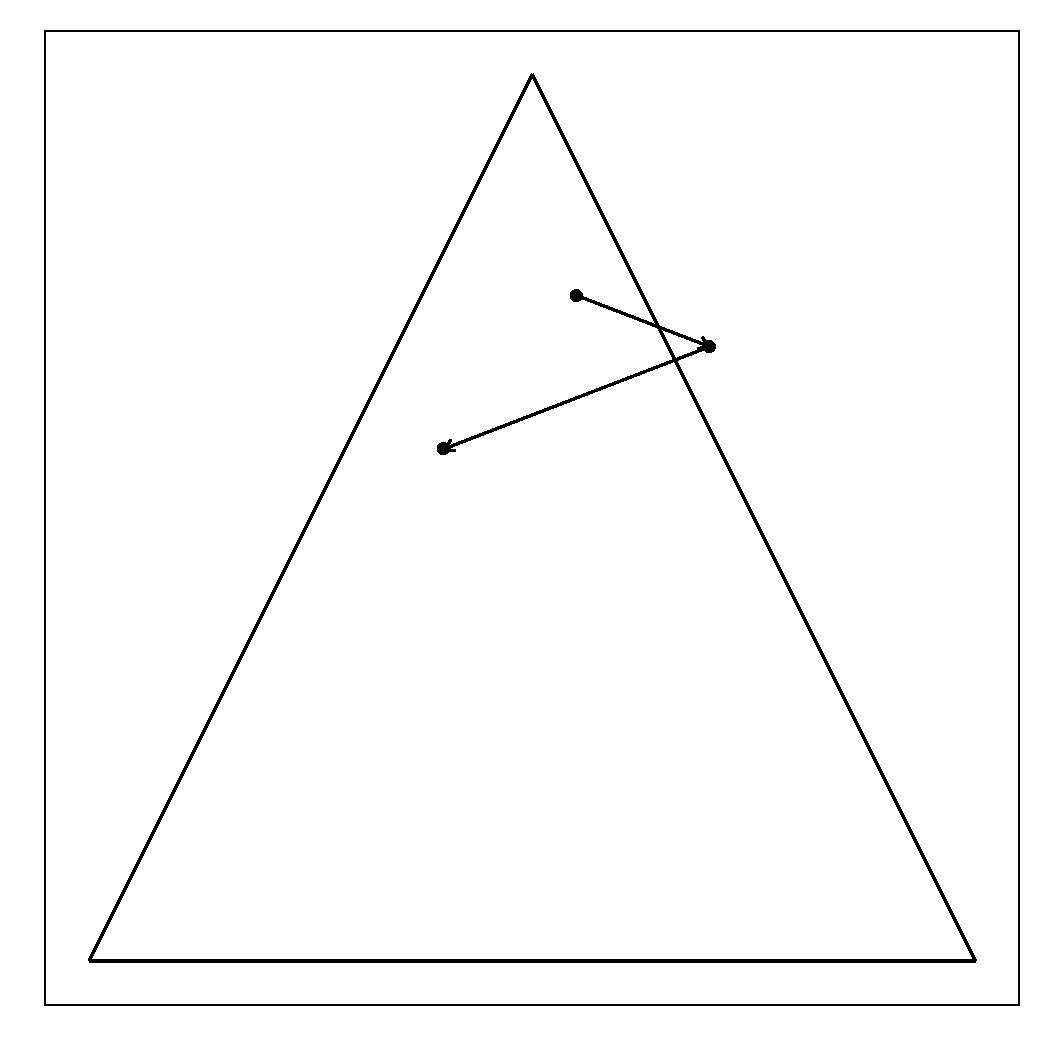
\includegraphics[width=\maxwidth]{figure/mirror_walkthrough3} 

\end{knitrout}

\caption{The step from Figure 14 is then repeated.}
\end{figure}

\end{document}
